\chapter{INTERFACE DEVELOPED FOR THE BLENDER GAME ENGIME}

% introduction
\section{Introduction}

% video game history
Video games have been around since the 1950s\cite{computerVideoGamesHistory}. They became available in the market by the 1970s, at that time they were very popular. Currently, games are the attraction of many people. They are all kinds of game available now. They are available for consoles, portable consoles, computer, cell phones; games are everywhere. 

% our aim
Our intention is to create tools that helps to create games but not any kind of games, we focus in \textit{educational games}. Educational games are the games that not only the player enjoy while he/she is playing moreover the player also learn playing it. Therefore we chose \textit{Blender} as the software to enhance in this project. We would be working on it \textit{Game Engine} which lacks of Particle Systems.

% layout of the chapter
This chapter goes as follows, we are going to briefly discuss what is \textit{Blender}, following by a description of its \textit{Game Engine}. Then, we are going to present the Boids particle system outside the Blender Game Engine, and finally we would present the custom modifier developed for the use of the RTPS library.

% blender background info
\section{Blender}\label{blenderSec}
\textit{Blender}\footnote{http://www.blender.org} is a free modeling/simulation software that has been out since 1993, it was most used to create 2D and 3D content. Currently, it has been extended and it can also do modeling, texturing, animation, particle simulation, rendering, game creation, etc.

When searching for the right software to use the following properties of Blender made it the top software in the list. Blender has a free game engine built-in, it can be extended (Open Source project), it is cross-platform i.e. it can be used in either Windows, MacOSX and Linux, and that it can support simulations with real physics. Blender also has a big support from the gaming industry, and there is a large community helping with tutorials and documentation for either beginners or technical functionality of Blender.

% game engine
\section{Game Engines}

% what is a game engine?
A game engine is a software or part of a software that simulates part of reality\cite{bookGameKit2}. Game engines let you interact with 3D world in real-time. Also, you can control objects that interact with other objects in the world. A game engine consist of several parts:
\begin{enumerate}
\item{render the 3D world and the objects on it}
\item{rerender the scenes when something in the world changes}
\item{game logic, decide what to do when the game is been play}
\item{simulates the physics of the game i.e. gravity}
\item{collision detection and reaction}
\end{enumerate}

Game engines would try to simulates these parts as quick as possible, so the game has a smooth fluency. Game engines are much more complicated than this, here we just mentioned a few of the most important parts that characterize them.

% blender game engine
As we mentioned in section~\ref{blenderSec} Blender has a \textit{Game Engine} built-in. The Blender Game Engine is a very powerful tool, it allows games to be created without  the need for explicit programming. With its GUI you are able to create simple games just by clicking and dragging. After creating the 3D objects and 3D world you can use the simple logic editor to bring the scene to life. The logic editor interface is shown in Figure~\ref{logic}.

\begin{figure}[htbp]
\begin{center}
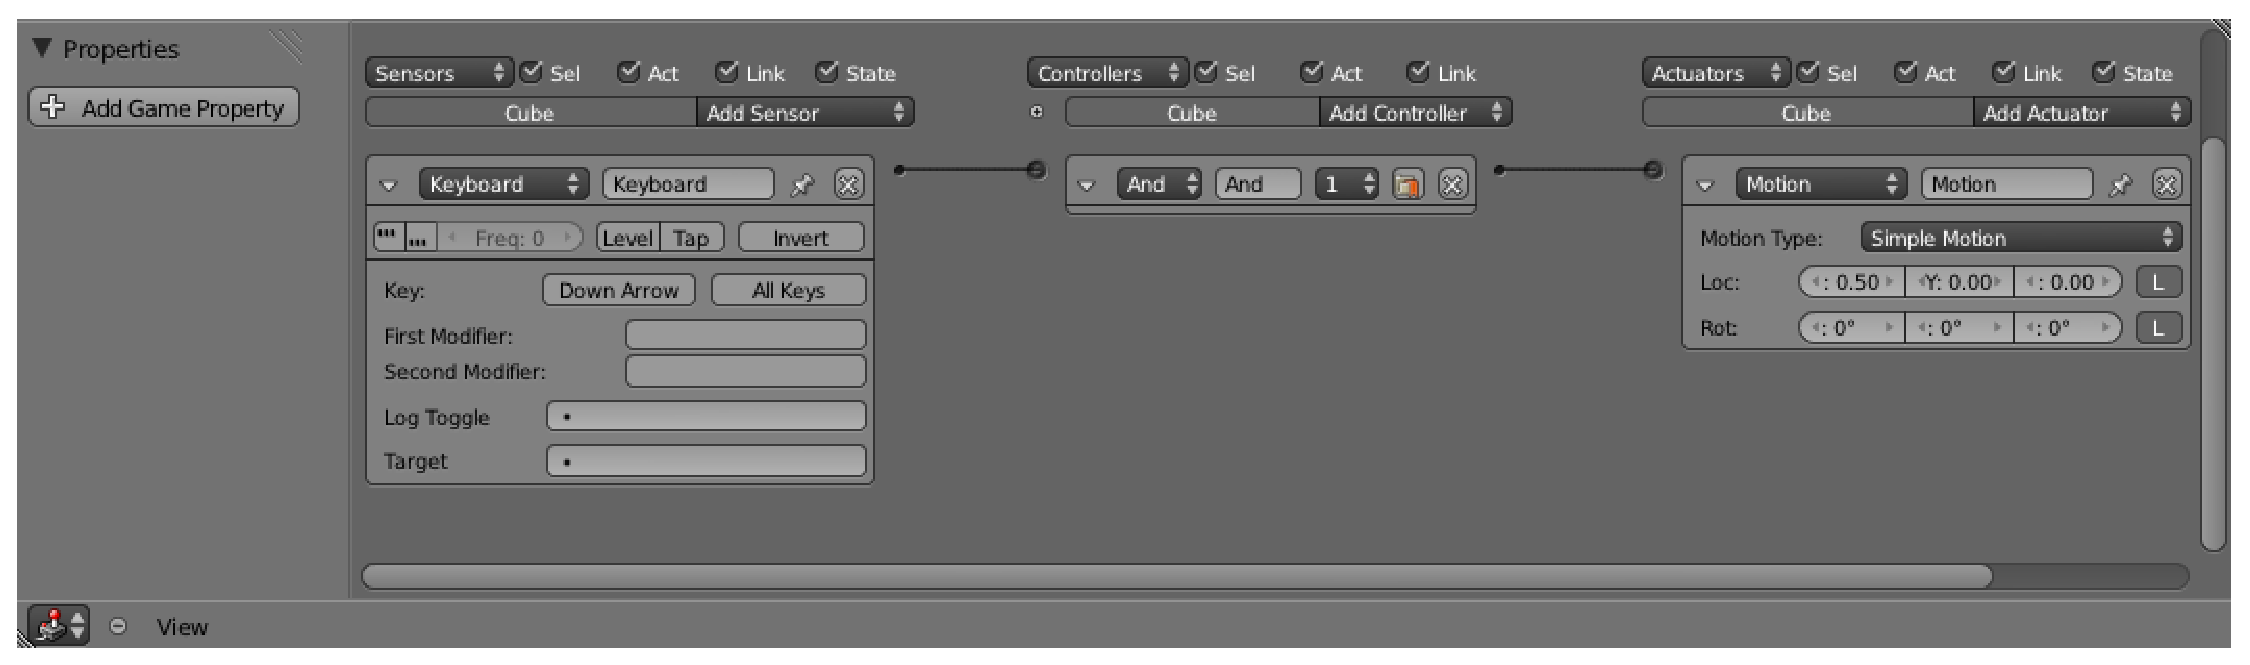
\includegraphics[scale=0.4]{figures/logic.eps}
\caption{Blender Game Engine Logic Editor interface}
\label{logic}
\end{center}
\end{figure}

The logic editor interface consists in two parts: \textit{Properties} and \textit{Logic Bricks}. Properties are used to give more specific actions to the objects, this properties can be called using the variable's names. The name of the variables has to match with the specific implementation in the source code. The second part are the logic bricks. The logic bricks are divided in \textit{sensors}, \textit{controllers}, and \textit{actuators}. Each of this has different subtypes to chose from.

Sensors are used to detect the input from the user e.g. sensors can be from the keybord, mouse, joysticks, etc. Controllers link the Sensors with the Actuators, using Controllers you can decide what action to take after the input has been received. The Actuators would make the actual action within the game. As an example the object might move, rotate, create, destroyed, change in shape, etc.

To create logic for an object in the world you just have to add as many logic bricks you need, and do not forget to connect them by dragging the connector from the sensor to the controller and from the controller to the actuator. The example move showed in Figure~\ref{logic} shows the forward movement of a cube using the down arrow.

This is the simplest way to create life within the world. For more complex behavior you can extend the capabilities by using Python scripting by using the Python scripting interface.

% particle system outside the blender game engine
\section{Boids Particle System outside the Blender Game Engine}
Although Blender has extensive particle-based tools, including hair styling, these are absent from the Game Engine. A submodule of the particle system is a rather sophisticated Boid system. In this section we would present how this Boid system works.

First you would need to create a particle emitter, it can be a cube, a plane, or any other object. Then, you make that object a particle system. Figure~\ref{boidsCreatePS} shows the panel used to add the particle system. The amount of particles is set to 50, using the starting and ending time as 1 would make the simulation to be calculate at each time step, there is no repetition (oscillation) in the movement of the boids, the lifetime is set to a big number to keep our boids a life for long time, using these settings would as much as we can do for real-time like simulation using the Boids system of Blender.

% figure: create PS
\begin{figure}[htbp]
\begin{center}
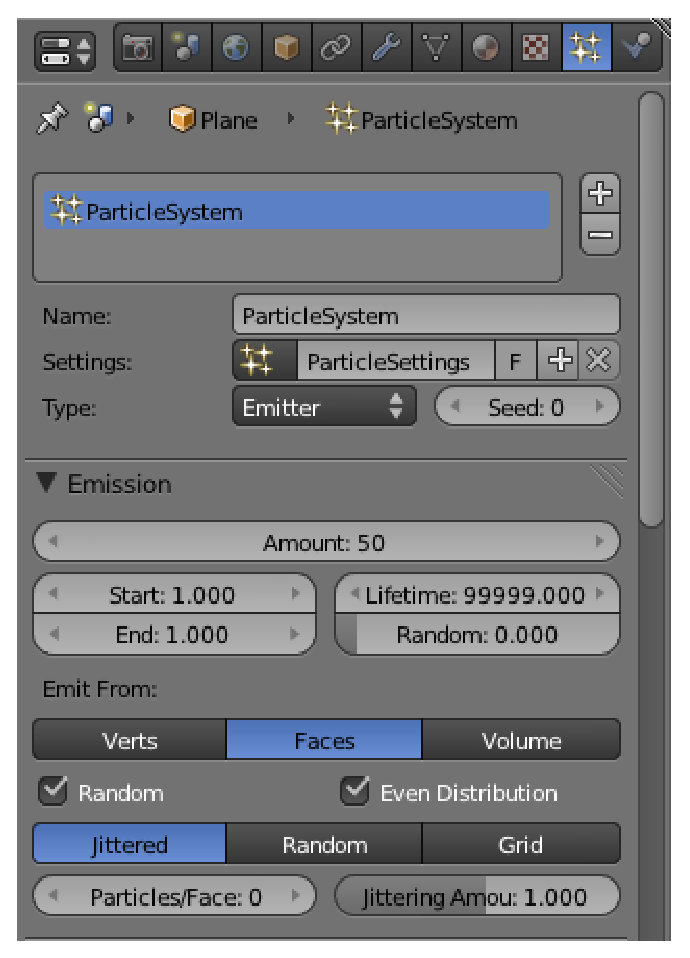
\includegraphics[scale= 0.5]{figures/boidsCreatePS.eps} 
\caption{Blender Particle Systems Add/Emission panel}
\label{boidsCreatePS}
\end{center}
\end{figure}

After the system is created, we can edit the physics of it, see Figure~\ref{boidsPhysics}. First, we click on \textit{Boids}, and all the settings of the system show up. The default Blender particle system is Newtonian. Settings can be changed dynamically while the animation is running.

% figure: boids physics
\begin{figure}[htbp]
\begin{center}
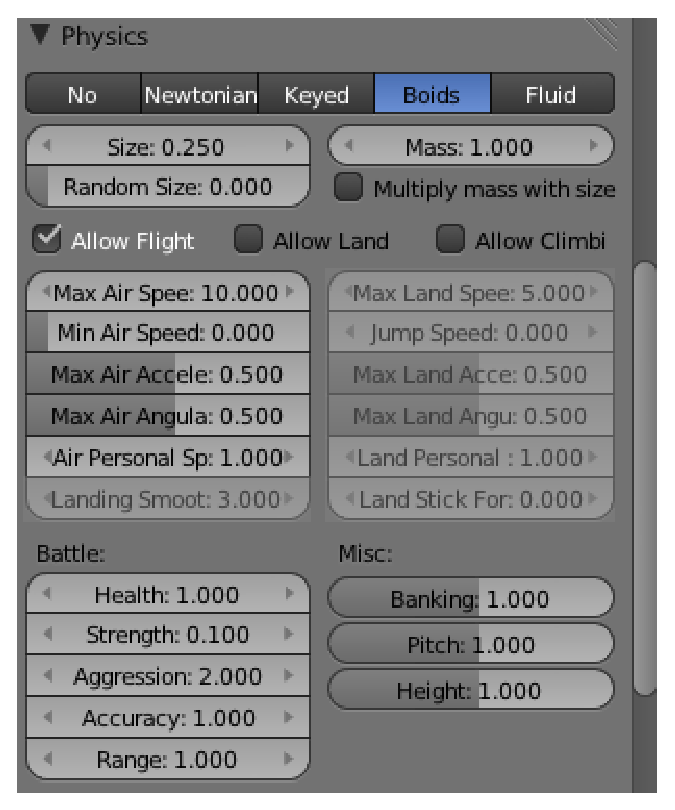
\includegraphics[scale = 0.5]{figures/boidsPhysics.eps} 
\caption{Blender Particle Systems Physics panel}
\label{boidsPhysics}
\end{center}
\end{figure}

Each boid has its own brain, therefore their actions are evaluated individually. Figure~\ref{boidsBrain} shows the panel for the Boid Brain. Let us first discuss the rules available in Blender.

%Blender boid's rules
\begin{enumerate}
\item{Goal: }
\item{Avoid: }
\item{Avoid Collision: }
\item{Separate: }
\item{Flock: }
\item{Follow Leader: }
\item{Average Speed: }
\item{Fight: }
\end{enumerate}

When clicking in a rule, if that rule needs some extra parameters, the respective input areas are going to show up. As can be seen in Figure~\ref{boidsBrain}, after clicking the rule Goal the options of which object is going to be target shows, we set it to the empty object target which was created by us. They are three ways available to evaluate the rule: fuzzy logic with a fuzziness level, averaging all rules, and weighting the rules randomly. Each of these evaluations leads to completely different results. The type of evaluation that is most commonly used is Fuzzy.

The render panel can be also seen in Figure~\ref{boidsBrain}. We changed the rendering type to object and set a monkey to be the object to be render as a boid.

% figure: boid brain
\begin{figure}[htbp]
\begin{center}
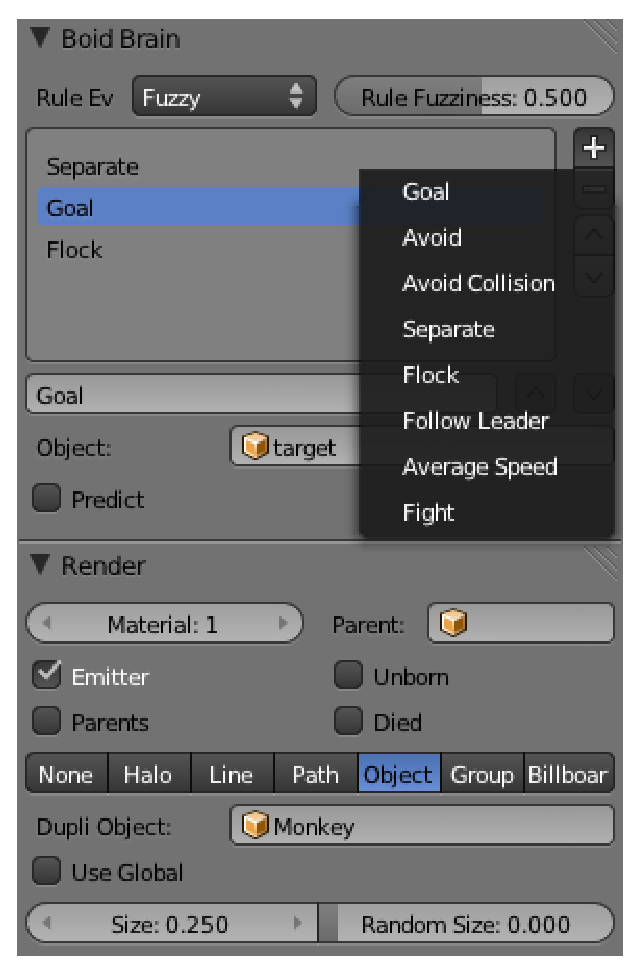
\includegraphics[scale = 0.5]{figures/boidsBrain.eps}
\caption{Blender Particle Systems Boid Brain panel}
\label{boidsBrain}
\end{center}
\end{figure}

Figure~\ref{boidsAction} shows two screenshots of an animation in which the boids are approaching an empty object as the target. This animation was ran using the settings presented in the previous Figures.

% figure: boids in action
\begin{figure}[htbp]
\begin{center}$
\begin{array}{cc}
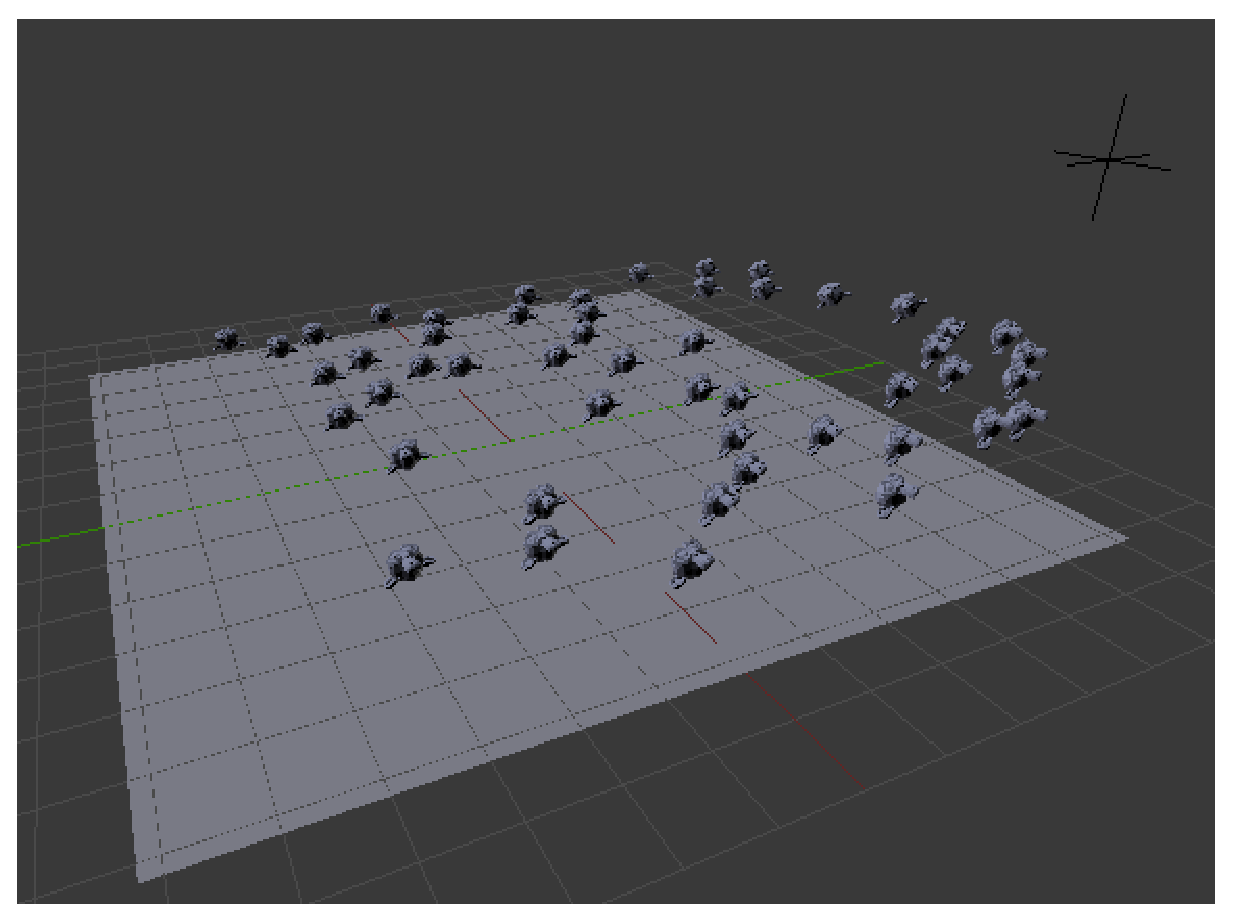
\includegraphics[scale= 0.35]{figures/boids1.eps} &
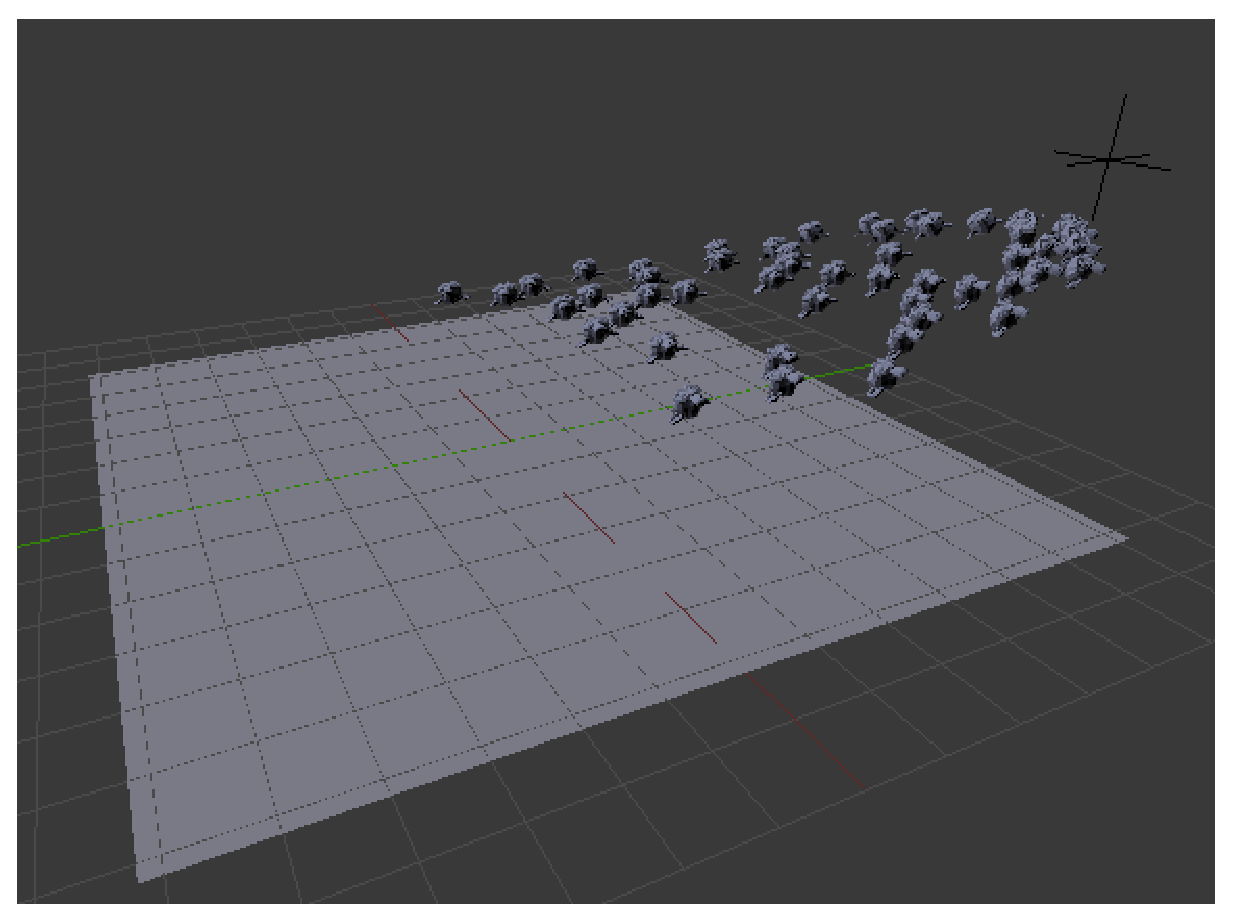
\includegraphics[scale= 0.35]{figures/boids2.eps}
\end{array}$
\end{center}
\caption{Screenshots of the boids approaching the target}
\label{boidsAction}
\end{figure}

% RTPS modifier
\section{RTPS Custom Modifier}
In this section we are going to present the 

% code modifications
\subsection{Game Engine Source Code Modifications}

% UI
\subsection{Development of the UI}

